\begin{figure*}[htbp]
    \centering
    % Row 1
    \begin{subfigure}[b]{0.22\textwidth}
        \centering
        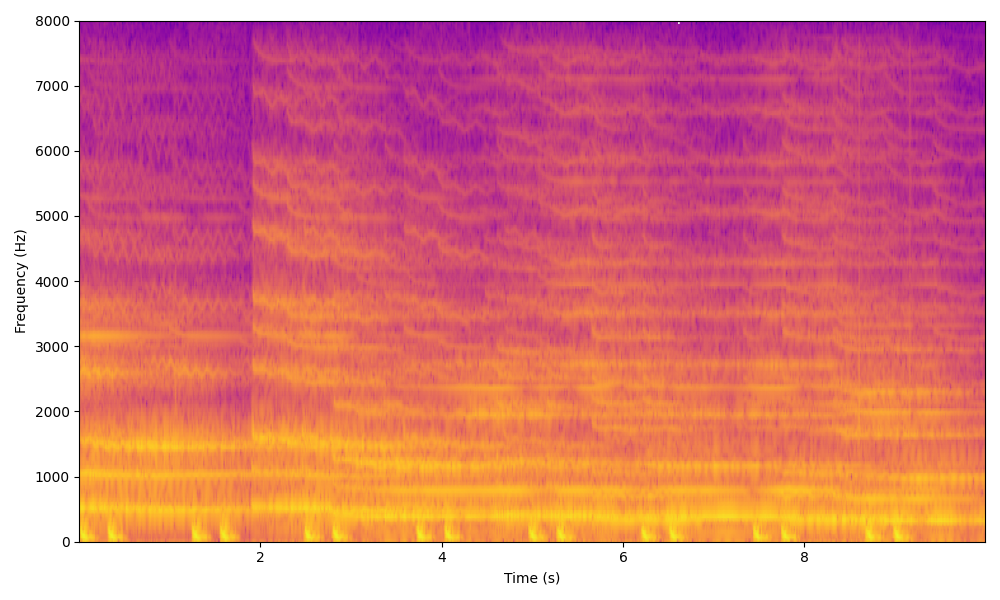
\includegraphics[width=\textwidth]{plots/onepeace_best_sdr/onepeace mixture_spectrogram.png}
        \caption*{Mixture}
    \end{subfigure}
     \begin{subfigure}[b]{0.22\textwidth}
        \centering
        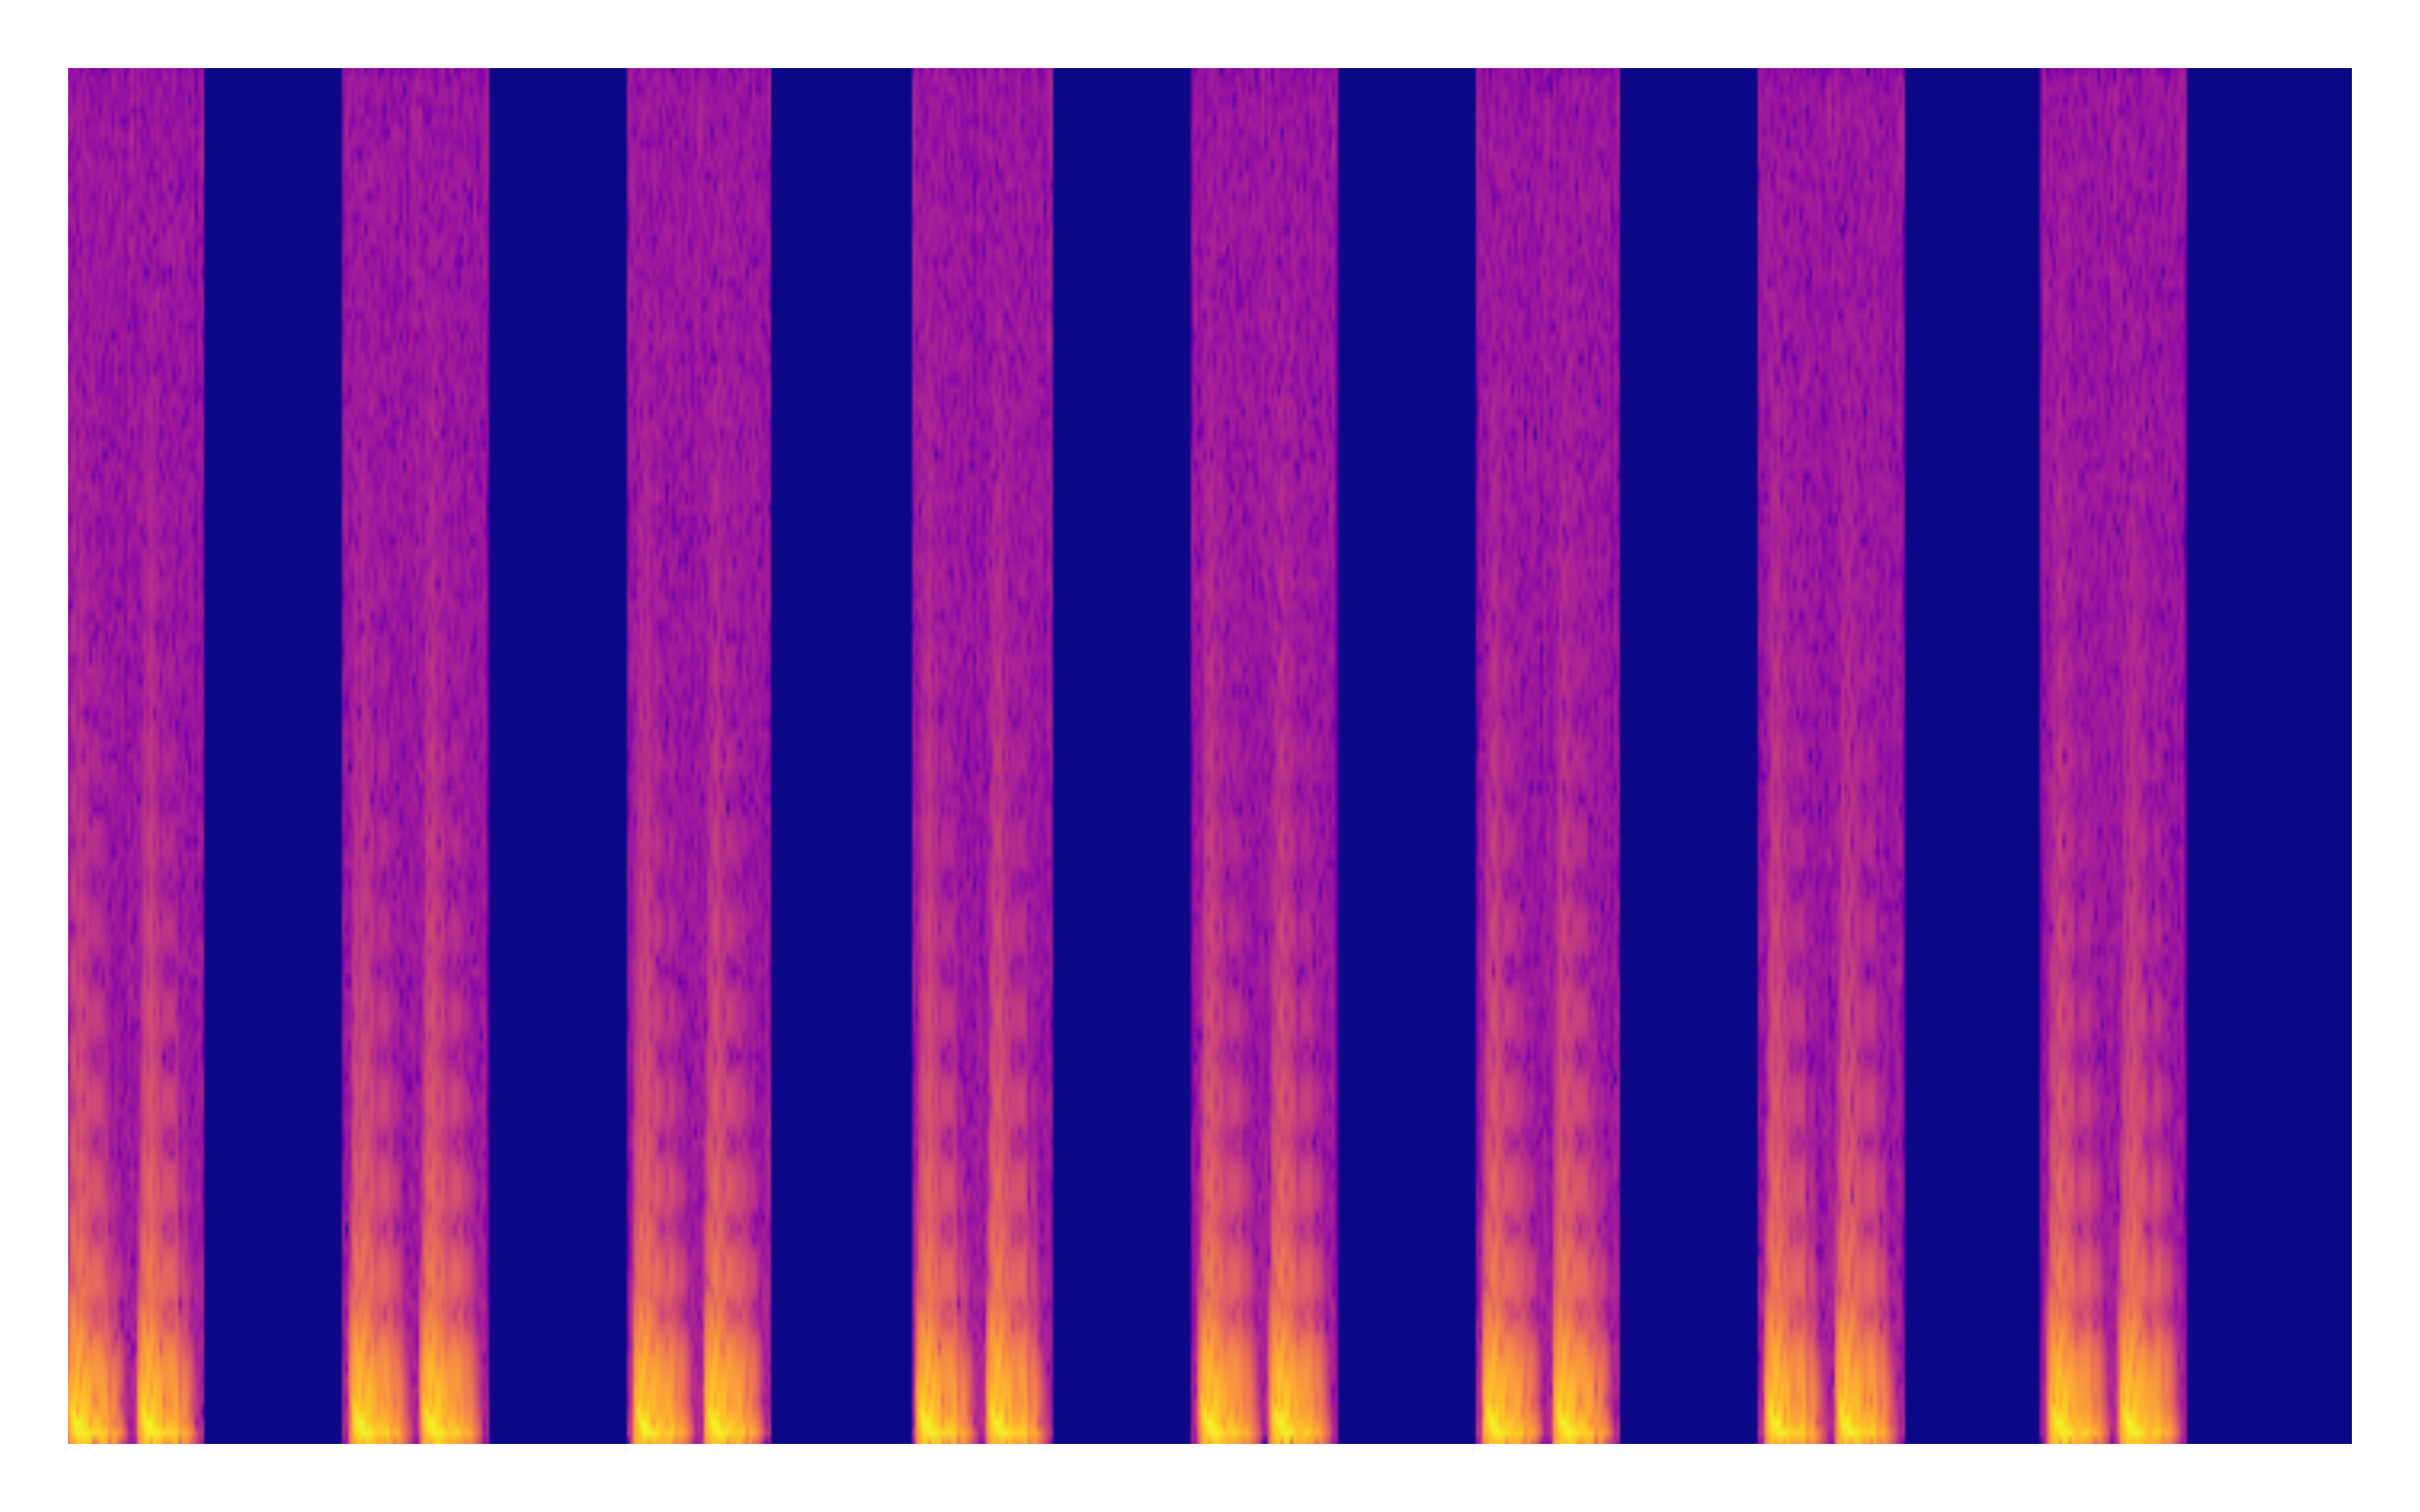
\includegraphics[width=\textwidth]{plots/onepeace_best_sdr/onepeace target_spectrogram.png}
        \caption*{Target}
    \end{subfigure}
    \begin{subfigure}[b]{0.22\textwidth}
        \centering
        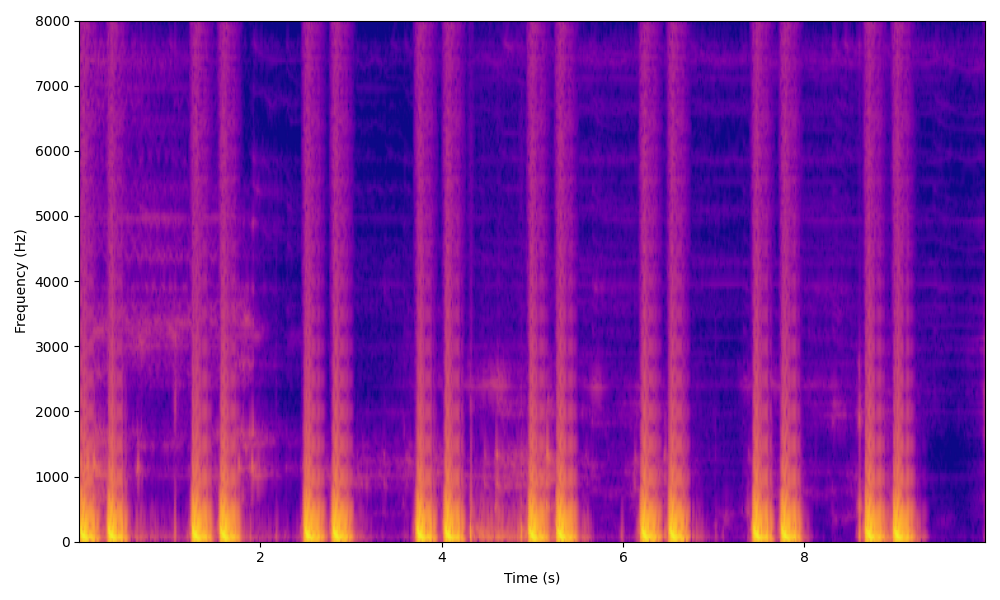
\includegraphics[width=\textwidth]{plots/onepeace_best_sdr/onepeace sep_spectrogram.png}
        \caption*{Separation Result\\(One-Peace)}
    \end{subfigure}
    \begin{subfigure}[b]{0.22\textwidth}
        \centering
        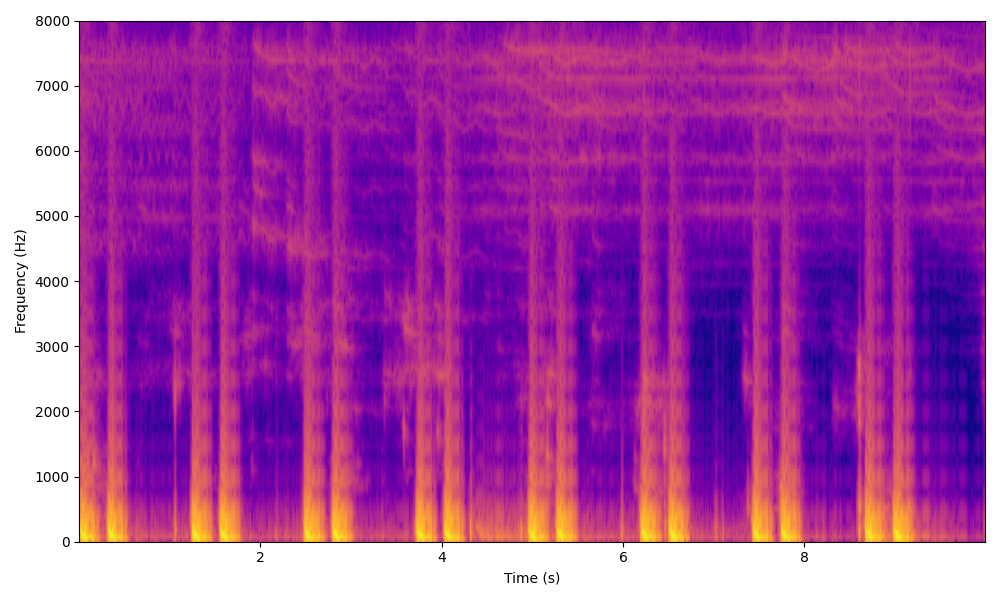
\includegraphics[width=\textwidth]{plots/onepeace_best_sdr/clap sep_spectrogram.png}
        \caption*{Separation Result\\(CLAP)}
    \end{subfigure}

    % % Row 2
    % \begin{subfigure}[b]{0.3\textwidth}
    %     \centering
    %     \includegraphics[width=\textwidth]{mixture_dog.png}
    %     \caption*{Mixture}
    % \end{subfigure}
    % \begin{subfigure}[b]{0.3\textwidth}
    %     \centering
    %     \includegraphics[width=\textwidth]{separation_dog.png}
    %     \caption*{Separation Result}
    % \end{subfigure}
    % \begin{subfigure}[b]{0.3\textwidth}
    %     \centering
    %     \includegraphics[width=\textwidth]{target_dog.png}
    %     \caption*{Target}
    % \end{subfigure}

    % Continue rows similarly for other queries
    % Add caption below
    \caption{Spectrogram results for various text queries. The first column shows the mixture, the second column shows the separation results, and the third column shows the target.}
    
    \label{fig:separation_results}

\end{figure*}
